\SGASection{3}{Scheme of parabolic subgroups of a reductive group}
\SGARefTarget{sga3:xxvi:section:3}

\SGAInlineRefTarget{sga3:xxvi:paragraph:3-1}\paragraph{\SGARefLink{sga3:xxvi:paragraph:3-1}{3.1}.}
Let \(E\) be a finite twisted constant \(S\)-scheme (Exp.\ X, \SGARefLink{sga3:x:definition:5-1}{5.1}).
Consider the \(S\)-functor \(\Of(E)\), where \(\Of(E)(S')\) is the set of
open-and-closed subschemes of \(E_{S'}\), or equivalently the set of
open-and-closed subsets of \(E_{S'}\).  Then \(\Of(E)\) is representable
by a finite twisted constant \(S\)-scheme.  Indeed, if \(E=A_S\), for a
finite set \(A\), then
\[
 \Of(E)\simeq\mathcal P(A)_S,
\]
where \(\mathcal P(A)\) denotes the power set of \(A\); the general case
follows by descent of open-and-closed subschemes.  Plainly,
\[
 \Of(E_{S'})=\Of(E)_{S'},
 \qquad
 \Of(E\times_SE')=\Of(E)\times_S\Of(E').
\]
\SGARefTarget{sga3:xxvi:item:3:1}

\paragraph{\SGARefLink{sga3:xxvi:item:3:1}{3.2}.}
Let \(S\) be a scheme and \(G\) an \(S\)-reductive group.  Define the
functor \(\Par(G)\) of parabolic subgroups of \(G\) by
\[
 \Par(G)(S')
 =\{\text{parabolic subgroups of }G_{S'}\}.
\]
In particular \(G\in\Par(G)(S)\), and
\(\underline{\operatorname{Bor}}(G)\subset\Par(G)\).  We shall define a
morphism
\[
 t:\Par(G)\longrightarrow\Of(\underline{\operatorname{Dyn}}(G))
\]
with the following properties:
\begin{enumerate}[label=\textup{(\roman*)}]
\item \(t\) is functorial in \(G\), with respect to isomorphisms, and
commutes with base change.
\item If \((T,M,R,\Delta,\ldots)\) is a pinning of \(G\) adapted to a
parabolic subgroup \(P\), then the canonical isomorphism
\[
 \underline{\operatorname{Dyn}}(G)\simeq\Delta_S
\qquad\textup{(Exp.\ XXIV, 3.4(iii))}
\]
carries \(t(P)\) onto \(\Delta(P)_S\), in the notation of \SGARefLink{sga3:xxvi:definition:1-11}{1.11} and \SGARefLink{sga3:xxvi:proposition:1-12}{1.12}.
\end{enumerate}

First suppose that \(P\) is a parabolic subgroup of \(G\) and that
\((T,M,R,\Delta,\ldots)\) is a pinning of \(G\) adapted to \(P\).  Define
\(t(P)\) by (ii).  The resulting subscheme of
\(\underline{\operatorname{Dyn}}(G)\) is independent of the pinning.
Indeed, if \((T',M',R',\Delta',\ldots)\) is another pinning adapted to
\(P\), then the unique inner automorphism of \(G\) carrying the first
pinning to the second comes from \(P\), by \SGARefLink{sga3:xxvi:prop:1:15}{1.15}.  The canonical
isomorphism \(\Delta\xrightarrow{\sim}\Delta'\) therefore carries
\(\Delta(P)\) onto \(\Delta'(P)\).

Without assuming that \((G,P)\) admits a pinning, \SGARefLink{sga3:xxvi:lemma:1:14}{1.14} and the definition
of \(\underline{\operatorname{Dyn}}(G)\) (Exp.\ XXIV, \SGARefLink{sga3:xxiv:3.3}{3.3}) allow one to
descend a unique open-and-closed subscheme \(t(P)\) such that
\[
 t(P)_{S'}=t(P_{S'})
\]
whenever \((G,P)_{S'}\) admits a pinning.
\SGARefTarget{sga3:xxvi:item:3:2}

\begin{sgastatement}{Theorem 3.3}
Let \(S\) be a scheme, \(G\) an \(S\)-reductive group, and
\[
 t:\Par(G)\longrightarrow\Of(\underline{\operatorname{Dyn}}(G))
\]
the morphism just defined.
\begin{enumerate}[label=\textup{(\roman*)}]
\item Two parabolic subgroups \(P,P'\) of \(G\) are conjugate locally for
the fpqc topology \textup{(cf.\ \SGARefLink{sga3:xxvi:proposition:1-3}{1.3})} if and only if \(t(P)=t(P')\).
\item\SGAInlineRefTarget{sga3:xxvi:thm:3:3:item:ii} \(\Par(G)\) is representable, and \(t\) is smooth and projective,
with integral geometric fibers.
\end{enumerate}
\end{sgastatement}
\SGARefTarget{sga3:xxvi:thm:3:3}

By 3.2(i), together with the fact that inner automorphisms of \(G\) act
trivially on \(\underline{\operatorname{Dyn}}(G)\)
(Exp.\ XXIV, \SGARefLink{sga3:xxiv:3.4:item:iv}{3.4(iv)}), conjugate parabolics have the same type.
Conversely, suppose \(t(P)=t(P')\).  Locally one may first assume that
both \((G,P)\) and \((G,P')\) admit pinnings (\SGARefLink{sga3:xxvi:lemma:1:14}{1.14}).  By the conjugacy of
pinnings in \(G\) (Exp.\ XXIV, \SGARefLink{sga3:xxiv:1.5}{1.5}), one may then choose a single pinning
\((T,M,R,\Delta)\) adapted to both \(P\) and \(P'\).  Equality of types
gives \(\Delta(P)=\Delta(P')\), hence \(P=P'\) by \SGARefLink{sga3:xxvi:prop:1:4:item:v}{1.4(v)}.  This proves
(i).

For (ii), use the notation of Exp.\ XXII, \SGARefLink{sga3:xxii:prop:5.11.5}{5.11.5}.
There is a canonical morphism \(\Par(G)\to\mathscr H_c\), which fits into
the cartesian square
\[
\begin{tikzcd}[column sep=large,row sep=large]
 \Par(G) \arrow[r,"t"] \arrow[d,hook]
   & \Of(\underline{\operatorname{Dyn}}(G)) \arrow[d,hook]\\
 \mathscr H_c \arrow[r,"c\ell"]
   & \mathcal C\ell_c .
\end{tikzcd}
\]
The vertical arrows are monomorphisms.  By \emph{loc.\ cit.},
\(\mathscr H_c\) is representable and \(c\ell\) is smooth,
quasi-projective, and of finite presentation, with integral geometric
fibers; hence the same is true of \(t\).

It remains to prove that \(t\) is proper.  This is fpqc-local, so one may
reduce to a pinned group \(G=(G,T,M,R,\Delta,\ldots)\).  Then
\(\underline{\operatorname{Dyn}}(G)\simeq\Delta_S\), and it is enough to
show that
\[
 t^{-1}((\Delta_1)_S)
\]
is proper over \(S\) for every \(\Delta_1\subset\Delta\).  Let \(P_1\)
be the parabolic containing \(T\) with \(\Delta(P_1)=\Delta_1\).  Part
(i) shows that \(g\mapsto\Int(g)P_1\) induces an isomorphism
\[
 G/\Norm_G(P_1)\xrightarrow{\sim}t^{-1}((\Delta_1)_S).
\]
By \SGARefLink{sga3:xxvi:prop:1:2}{1.2}, \(G/\Norm_G(P_1)=G/P_1\), which is projective over \(S\).

\begin{sgastatement}{Definition 3.4}
\(\Of(\underline{\operatorname{Dyn}}(G))\) is called the
\emph{scheme of types of parabolics} of \(G\), and \(t(P)\) is called
the \emph{type} of \(P\).
\end{sgastatement}
\SGARefTarget{sga3:xxvi:def:3:4}

\begin{sgastatement}{Corollary 3.5}
The \(S\)-functor \(\Par(G)\) is representable by an \(S\)-scheme that is
smooth and projective over \(S\).  The factorization
\[
 \Par(G)\longrightarrow
 \Of(\underline{\operatorname{Dyn}}(G))
 \longrightarrow S
\]
is the Stein factorization \textup{(EGA III, 4.3.3)} of the structural
morphism \(\Par(G)\to S\).
\end{sgastatement}
\SGARefTarget{sga3:xxvi:cor:3:5}

\begin{sgastatement}{\SGAInlineRefTarget{sga3:xxvi:corollary:3-6}Corollary 3.6}
For every
\(t\in\Of(\underline{\operatorname{Dyn}}(G))(S)\), the \(S\)-scheme
\[
 \Par_t(G)=t^{-1}(t)
\]
of parabolic subgroups of type \(t\) is smooth and projective over \(S\)
and homogeneous under \(G\).  If \(P\) is a parabolic subgroup of \(G\),
there is a canonical isomorphism
\[
 G/P\xrightarrow{\sim}\Par_{t(P)}(G).
\]
Moreover,
\[
 \Par_{\varnothing}(G)=\underline{\operatorname{Bor}}(G),
 \qquad
 \Par_{\underline{\operatorname{Dyn}}(G)}(G)\xrightarrow{\sim}S.
\]
\end{sgastatement}
\SGARefTarget{sga3:xxvi:cor:3:6}

\begin{sgastatement}{\SGAInlineRefTarget{sga3:xxvi:remark:3-7}Remark 3.7}
The \(S\)-scheme \(\Of(\underline{\operatorname{Dyn}}(G))\) has a natural
order structure, the domination relation being set-theoretic inclusion of
subschemes.  It is a lattice; in particular, the infimum of two
open-and-closed subschemes of
\(\underline{\operatorname{Dyn}}(G)_{S'}\) is their intersection.

If \(B\) is a Borel subgroup of \(G\), let \(X\) be the functor of
parabolic subgroups containing \(B\).  The morphism
\[
 X\longrightarrow\Of(\underline{\operatorname{Dyn}}(G))
\]
induced by \(t\) is an isomorphism of ordered schemes.  This follows from
\(P\subset Q\Rightarrow t(P)\subset t(Q)\) and the next lemma.
\end{sgastatement}
\SGARefTarget{sga3:xxvi:rem:3:7}

\begin{sgastatement}{Lemma 3.8}
Let \(S\) be a scheme, \(G\) an \(S\)-reductive group, \(P\) a parabolic
subgroup of \(G\), and
\[
 t'\in\Of(\underline{\operatorname{Dyn}}(G))(S)
\quad\text{with}\quad
 t(P)\subset t'.
\]
There is a unique parabolic subgroup \(P'\) of \(G\) containing \(P\)
and satisfying \(t(P')=t'\).
\end{sgastatement}
\SGARefTarget{sga3:xxvi:lemma:3:8}

After extending the base, one may suppose that \(P\) contains a Borel
subgroup \(B\) of \(G\).  Uniqueness then follows from \SGARefLink{sga3:xxvi:prop:1:17}{1.17}.  For
existence one may work in the split case, where the assertion is immediate
from §1.

\begin{sgastatement}{Remarks 3.8.1}
\begin{enumerate}[label=\textup{(\roman*)}]
\item The analogue of \SGARefLink{sga3:xxvi:lemma:3:8}{3.8} obtained by reversing the inclusions is false.
It would imply, for example, that every group of type \(A_1\) has a Borel
subgroup, which is not so \textup{(Exp.\ XX, §5)}.
\item The preceding discussion shows that \(t(P)\subset t(Q)\) means that
locally for the fpqc, or étale, topology, \(P\) is conjugate to a subgroup
of \(Q\).  It is enough to check this on geometric fibers.  \SGARefLink{sga3:xxvi:section:5}{Section~5}
will show that the étale topology may be replaced by the Zariski topology.
\end{enumerate}
\end{sgastatement}
\SGARefTarget{sga3:xxvi:rem:3:8:1}

\SGAInlineRefTarget{sga3:xxvi:paragraph:3-9}\paragraph{\SGARefLink{sga3:xxvi:paragraph:3-9}{3.9}.}
The preceding discussion can be repeated for critical subgroups.  Recall
(Exp.\ XXII, \SGARefLink{sga3:xxii:def:5.10.4}{5.10.4} and \SGARefLink{sga3:xxii:cor:5.10.5}{5.10.5}) that a reductive subgroup \(H\) of a
reductive group \(G\) is \emph{critical} if
\[
 H=\Centr_G(\rad(H)),
\]
that a subtorus \(Q\subset G\) is a \emph{\(C\)-critical torus} if
\[
 Q=\rad(\Centr_G(Q)),
\]
and that critical subgroups and \(C\)-critical tori are in bijection via
\[
 H\longmapsto\rad(H),
 \qquad
 Q\longmapsto\Centr_G(Q).
\]

If \((G,T,M,R)\) is split, the subgroup of \(G\) containing \(T\) and
corresponding to \(R'\subset R\) (Exp.\ XXII, \SGARefLink{sga3:xxii:def:5.4.2}{5.4.2}) is critical if and
only if \(R'\) is \emph{vectorial}, meaning that it is the intersection
of \(R\) with a vector subspace of \(M\otimes\mathbb Q\)
(Exp.\ XXII, \SGARefLink{sga3:xxii:prop:5.10.6}{5.10.6}).

For arbitrary \(G\), Exp.\ XXII, \SGARefLink{sga3:xxii:prop:5.11.5}{5.11.5} defines a finite étale \(S\)-scheme
\(\mathcal C\ell_{\mathrm{crit}}\); in the split case it is the constant
scheme associated with the vectorial subsets of \(R\), modulo the action
of the Weyl group.  If \(\Crit(G)\) denotes the functor of critical
subgroups, there is a canonical morphism
\[
 c\ell:\Crit(G)\longrightarrow\mathcal C\ell_{\mathrm{crit}}
\]
in the cartesian square
\[
\begin{tikzcd}[column sep=large,row sep=large]
 \Crit(G) \arrow[r,"c\ell"] \arrow[d,hook]
   & \mathcal C\ell_{\mathrm{crit}} \arrow[d,hook]\\
  \mathscr H_c \arrow[r,"c\ell"]
   & \mathcal C\ell_c .
\end{tikzcd}
\]
\SGARefTarget{sga3:xxvi:item:3:9}

\begin{sgastatement}{Proposition 3.10}
Let \(S\) be a scheme, \(G\) an \(S\)-reductive group,
\(\Crit(G)\) the functor of its critical subgroups, and let
\(\mathcal C\ell_{\mathrm{crit}}\) and
\[
 c\ell:\Crit(G)\longrightarrow\mathcal C\ell_{\mathrm{crit}}
\]
be as above.
\begin{enumerate}[label=\textup{(\roman*)}]
\item Critical subgroups \(H,H'\) of \(G\) are conjugate, locally for the
fpqc topology, if and only if \(c\ell(H)=c\ell(H')\).
\item \(\Crit(G)\) is representable, and \(c\ell\) is smooth and affine,
with integral geometric fibers.
\end{enumerate}
\end{sgastatement}
\SGARefTarget{sga3:xxvi:prop:3:10}

The proof is the same as for \SGARefLink{sga3:xxvi:item:3:2}{3.3} except for affineness of \(c\ell\).  It
is enough to prove that \(\Crit(G)\) is affine over \(S\).
The functor \(\Crit(G)\) identifies naturally with the functor of critical
tori of \(G\), giving a canonical monomorphism
\[
 \Crit(G)\longrightarrow\mathcal M,
\]
where \(\mathcal M\) is the scheme of subgroups of multiplicative type of
\(G\) (Exp.\ XI, \SGARefLink{sga3:xi:theorem:4:1}{4.1}).  By Exp.\ XII, \SGARefLink{sga3:xii:5.3}{5.3}, it is enough to show that this
is an open-and-closed immersion.  After the base change
\(\mathcal M\to S\), this reduces to the following: if \(Q\) is a subgroup
of multiplicative type in \(G\), the \(S'\to S\) for which \(Q_{S'}\) is
a critical torus of \(G_{S'}\) are precisely those factoring through an
open-and-closed subscheme of \(S\).  The condition is the conjunction of:
\begin{enumerate}[label=\textup{(\arabic*)}]
\item \(Q\) is a torus;
\item once \(Q\) is a torus, the torus \(\rad(\Centr_G(Q))\) has the same
relative dimension as \(Q\).
\end{enumerate}
Both conditions are of the required kind.

\begin{sgastatement}{Corollary 3.11}
The \(S\)-functor \(\Crit(G)\) is representable by an \(S\)-scheme that
is smooth and affine over \(S\).
\end{sgastatement}
\SGARefTarget{sga3:xxvi:cor:3:11}

\begin{sgastatement}{Corollary 3.12}
Let \(H\) be a critical subgroup of the \(S\)-reductive group \(G\).
Then \(G/\Norm_G(H)\) and \(G/H\) are representable by \(S\)-schemes that
are affine and smooth over \(S\).
\end{sgastatement}
\SGARefTarget{sga3:xxvi:cor:3:12}

The first assertion follows from \SGARefLink{sga3:xxvi:cor:3:11}{3.11}, and the second from the first and
Exp.\ XXII, \SGARefLink{sga3:xxii:cor:5.10.2}{5.10.2}.

\begin{sgastatement}{Corollary 3.13}
Let \(Q\) be a subtorus of the \(S\)-reductive group \(G\).  Then
\(G/\Centr_G(Q)\) is representable by an \(S\)-scheme that is smooth and
affine over \(S\).  The same holds for \(G/\Norm_G(Q)\) when \(Q\) is a
critical subtorus of \(G\).
\end{sgastatement}
\SGARefTarget{sga3:xxvi:cor:3:13}

Indeed, \(H=\Centr_G(Q)\) is critical (Exp.\ XXII, \SGARefLink{sga3:xxii:cor:5.10.5}{5.10.5}), and when
\(Q\) is critical one has
\(\Norm_G(H)=\Norm_G(Q)\) (\emph{loc.\ cit.}, 5.10.8).

\SGAInlineRefTarget{sga3:xxvi:paragraph:3-14}\paragraph{\SGARefLink{sga3:xxvi:paragraph:3-14}{3.14}.}
The conjugacy of Levi subgroups of parabolic subgroups of \(G\) gives a
unique morphism
\[
 u:\Of(\underline{\operatorname{Dyn}}(G))
 \longrightarrow\mathcal C\ell_{\mathrm{crit}}
\]
such that, for every parabolic subgroup \(P\) and every Levi subgroup
\(L\subset P\),
\[
 c\ell(L)=u(t(P)),
\]
compatibly with every base change.
\SGARefTarget{sga3:xxvi:item:3:14}

\paragraph{\SGARefLink{sga3:xxvi:item:3:14}{3.15}.}
Let \(S\) be a scheme and \(G\) an \(S\)-reductive group.  Consider the
\(S\)-functors
\[
\begin{aligned}
 PL(S')={}&\{(P,L)\mid P\supset L,\ P\text{ parabolic in }G_{S'},\
                    L\text{ a Levi subgroup of }P\},\\
 PT(S')={}&\{(P,T)\mid P\supset T,\ P\text{ parabolic in }G_{S'},\
                    T\text{ a maximal torus of }P\},\\
 CT(S')={}&\{(C,T)\mid C\supset T,\ C\text{ critical in }G_{S'},\
                    T\text{ a maximal torus of }C\},\\
 PLT(S')={}&\{(P,L,T)\mid P\supset L\supset T,\ (P,T)\in PT(S'),\
                    L\text{ a Levi subgroup of }P\}.
\end{aligned}
\]
There are evident morphisms between these functors and
\(\Par(G),\Crit(G)\), and \(\Tor(G)\).  They form the following
commutative truncated cube.

\begin{figure}[htbp]
\centering
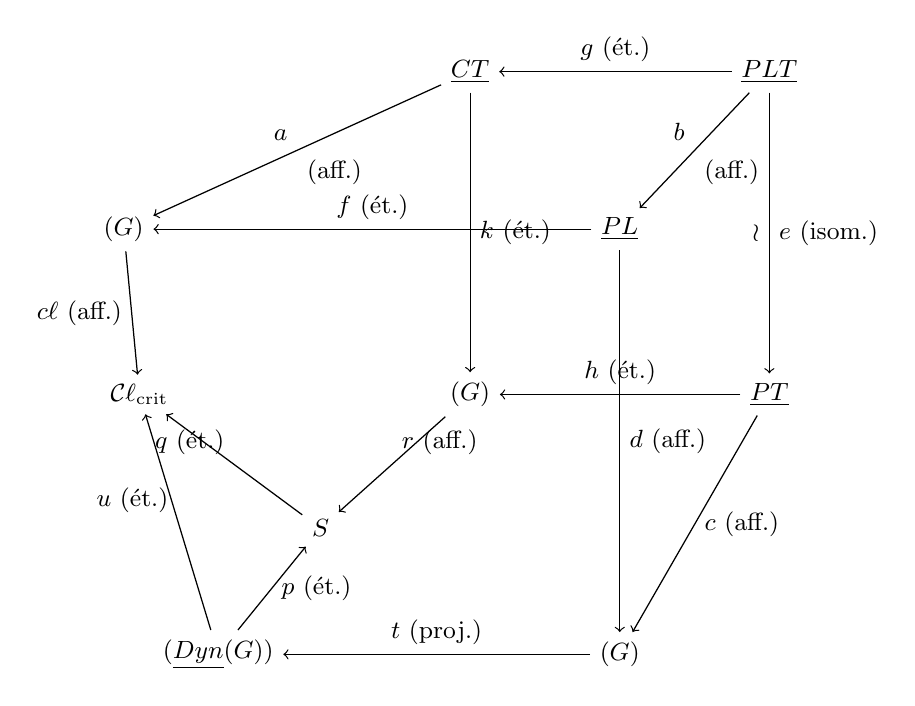
\begin{tikzpicture}[
  >=to,
  every node/.style={font=\small},
  morph/.style={->,line width=.45pt}
]
  \node (CT)     at (5.2,7.2) {\(\underline{CT}\)};
  \node (PLT)    at (9.0,7.2) {\(\underline{PLT}\)};
  \node (Crit)   at (0.8,5.2) {\(\Crit(G)\)};
  \node (PL)     at (7.1,5.2) {\(\underline{PL}\)};
  \node (Cl)     at (1.0,3.1) {\(\mathcal C\ell_{\mathrm{crit}}\)};
  \node (Tor)    at (5.2,3.1) {\(\Tor(G)\)};
  \node (PT)     at (9.0,3.1) {\(\underline{PT}\)};
  \node (S)      at (3.3,1.4) {\(S\)};
  \node (Of)     at (2.0,-.2) {\(\Of(\underline{\operatorname{Dyn}}(G))\)};
  \node (Par)    at (7.1,-.2) {\(\Par(G)\)};

  \draw[morph] (PLT) -- node[above]{\(g\) (ét.)} (CT);
  \draw[morph] (CT) -- node[above left]{\(a\)} node[below right]{(aff.)} (Crit);
  \draw[morph] (PLT) -- node[above left]{\(b\)} node[below right]{(aff.)} (PL);
  \draw[morph] (PL) -- node[above]{\(f\) (ét.)} (Crit);
  \draw[morph] (CT) -- node[right]{\(k\) (ét.)} (Tor);
  \draw[morph] (PLT) -- node[left]{\(\wr\)}
    node[right]{\(e\) (isom.)} (PT);
  \draw[morph] (Crit) -- node[left]{\(c\ell\) (aff.)} (Cl);
  \draw[morph] (PL) -- node[right]{\(d\) (aff.)} (Par);
  \draw[morph] (PT) -- node[above]{\(h\) (ét.)} (Tor);
  \draw[morph] (PT) -- node[right]{\(c\) (aff.)} (Par);
  \draw[morph] (S) -- node[above left]{\(q\) (ét.)} (Cl);
  \draw[morph] (Tor) -- node[above right]{\(r\) (aff.)} (S);
  \draw[morph] (Of) -- node[above left]{\(u\) (ét.)} (Cl);
  \draw[morph] (Of) -- node[right]{\(p\) (ét.)} (S);
  \draw[morph] (Par) -- node[above]{\(t\) (proj.)} (Of);
\end{tikzpicture}
\refstepcounter{figure}
\label{sga3:xxvi:fig:3:15:1}
\par\smallskip
{\small Figure 3.15.1}
\end{figure}
\SGARefTarget{sga3:xxvi:item:3:15}

\begin{sgastatement}{Theorem 3.16 \textup{(cf.\ Figure 3.15.1)}}
\begin{enumerate}[label=\textup{(\roman*)}]
\item Every morphism in the diagram is smooth, surjective, and of finite
presentation.
\item Every morphism except \(t\) is affine; \(t\) is projective.
\item Every morphism is either finite étale or has integral geometric
fibers: \(f,g,h,k,p,q,u\) are finite étale;
\(a,b,c,d,r,c\ell\) have integral geometric fibers; and \(e\) is an
isomorphism.
\item The square \((a,b,f,g)\) is cartesian.
\end{enumerate}
\end{sgastatement}
\SGARefTarget{sga3:xxvi:thm:3:16}

\SGAProof
It is clear from \SGARefLink{sga3:xxvi:proposition:1-6:item:ii}{1.6(ii)} that \(e\) is an isomorphism, and (iv) is
immediate.  The morphism \(a\) is smooth and affine with integral
geometric fibers.  Indeed, after the base change \(\Crit(G)\to S\), this
reduces to the same statement for
\[
 \Tor(L_0)\longrightarrow S,
\]
where \(L_0\) is the universal critical subgroup; \(L_0\) is reductive by
definition, so Exp.\ XXII, \SGARefLink{sga3:xxii:cor:5.8.3}{5.8.3} applies.  By (iv), \(b\) has the same
properties.

The morphism \(d\) is likewise smooth and affine with integral geometric
fibers, by \SGARefLink{sga3:xxvi:cor:1:9}{1.9}; the same is therefore true of
\[
 c=dbe^{-1}.
\]
The morphism \(r\) has these properties by Exp.\ XXII, \SGARefLink{sga3:xxii:cor:5.8.3}{5.8.3}, and
\(c\ell\) by \SGARefLink{sga3:xxvi:item:3:9}{3.10}.

We already know that \(p\) and \(q\) are finite étale and surjective
(\SGARefLink{sga3:xxvi:paragraph:3-1}{3.1} and \SGARefLink{sga3:xxvi:paragraph:3-9}{3.9}).  If \(f\) and \(k\) are finite étale and surjective, then
so is \(g\), by (iv), and so is \(h=kge^{-1}\).  Since the assertions
about \(t\) were proved in \SGARefLink{sga3:xxvi:thm:3:3:item:ii}{3.3(ii)}, it remains only to prove the claim for
\(f\) and \(k\).  We do so for \(k\), the proof for \(f\) being the same.

If \(T\) is a maximal torus of \(G\), let \(\mathcal C\) be the functor of
critical subgroups containing \(T\).  We must show that \(\mathcal C\) is
represented by a finite étale \(S\)-scheme with nonempty fibers.  We may
suppose that \(G\) is split relative to \(T\).  If \(E\) is the set of
vectorial subsets of the root system \(R\), then \(\mathcal C\) is
represented by \(E_S\), by 3.9.
\SGAQED

\begin{sgastatement}{Corollary 3.17}
All the functors in the preceding diagram are representable by
\(S\)-schemes that are smooth over \(S\), and all are affine over \(S\)
except \(\Par(G)\).
\end{sgastatement}
\SGARefTarget{sga3:xxvi:cor:3:17}

\begin{sgastatement}{\SGAInlineRefTarget{sga3:xxvi:remark:3-18}Remark 3.18}
\begin{enumerate}[label=\textup{(\roman*)}]
\item The fact that \(f:PL\to\Crit(G)\) is étale and surjective says that
a subgroup of \(G\) is critical if and only if, locally for the étale
topology, it is a Levi subgroup of a parabolic subgroup.

In general the map \(PL(S)\to\Crit(G)(S)\) need not be surjective: a
critical subgroup \(C\) may fail to arise over \(S\) from a parabolic
subgroup.  For example, a maximal torus need not be contained in a Borel
subgroup, as for a nonsplit form of \(\operatorname{SL}_2\)
\textup{(Exp.\ XX, §5)}.
\item Likewise,
\[
 u:\Of(\underline{\operatorname{Dyn}}(G))
 \longrightarrow\mathcal C\ell_{\mathrm{crit}}
\]
need not be an isomorphism.  Two parabolic subgroups of different types
may have Levi subgroups of the same type.  In a group of type \(A_2\),
for instance, the two types of parabolics whose Levi subgroups have
semisimple rank \(1\) correspond to the two vertices of the diagram,
whereas there is only one type of critical subgroup of rank \(1\).

The analogous example for type \(A_3\) shows that, even over an
algebraically closed field, nonisomorphic parabolic subgroups may have
Levi subgroups of the same type.\footnote{\emph{Editor's note.}
Concretely, in \(\operatorname{GL}_4\), the parabolics
\[
 P=\left\{\begin{pmatrix}
 *&*&*&*\\0&*&*&*\\0&0&*&*\\0&0&0&*
 \end{pmatrix}\right\},
 \qquad
 P'=\left\{\begin{pmatrix}
 *&*&*&*\\0&*&*&*\\0&*&*&*\\0&0&0&*
 \end{pmatrix}\right\}
\]
are not isomorphic (their unipotent radicals are not isomorphic), while
their Levi subgroups
\[
 L=\left\{\begin{pmatrix}
 *&*&0&0\\ *&*&0&0\\0&0&*&0\\0&0&0&*
 \end{pmatrix}\right\},
 \quad
 L'=\left\{\begin{pmatrix}
 *&0&0&0\\0&*&*&0\\0&*&*&0\\0&0&0&*
 \end{pmatrix}\right\}
\]
are conjugate by
\(
\left(\begin{smallmatrix}
0&0&1&0\\0&1&0&0\\1&0&0&0\\0&0&0&1
\end{smallmatrix}\right).
\)}
\end{enumerate}
\end{sgastatement}
\SGARefTarget{sga3:xxvi:rem:3:18}

We end this section with an application to principal bundles.

\begin{sgastatement}{\SGAInlineRefTarget{sga3:xxvi:lemma:3-20}Lemma 3.20}
Let \(S\) be a scheme, \(G\) an \(S\)-reductive group, \(F\) a principal
homogeneous bundle under \(G\), and \(G_F\) the corresponding twisted form.
Identify \(\underline{\operatorname{Dyn}}(G)\) with
\(\underline{\operatorname{Dyn}}(G_F)\) \textup{(Exp.\ XXIV, \SGARefLink{sga3:xxiv:3.5}{3.5})}.
For every parabolic subgroup \(P\) of \(G\), there is a canonical
isomorphism
\[
 F/P\xrightarrow{\sim}\Par_{t(P)}(G_F).
\]
In particular, the structural group of \(F\) reduces to \(P\) if and only
if \(G_F\) has a parabolic subgroup of type \(t(P)\).
\end{sgastatement}
\SGARefTarget{sga3:xxvi:lemma:3:20}

The proof is exactly the same as that of Exp.\ XXIV, \SGARefLink{sga3:xxiv:proposition:4-2-1}{4.2.1}.

\SGAInlineRefTarget{sga3:xxvi:paragraph:3-21}\paragraph{\SGARefLink{sga3:xxvi:paragraph:3-21}{3.21}.}
If \(S\) is a scheme, \(G\) an \(S\)-reductive group, and
\[
 t\in\Of(\underline{\operatorname{Dyn}}(G))(S),
\]
write \(H^1_t(S,G)\) for the subset of \(H^1(S,G)\) consisting of the
classes of principal \(G\)-bundles \(F\) for which the associated group
\(G_F\) has a parabolic subgroup of type \(t\).  If \(G\) itself has a
parabolic subgroup \(P\) of type \(t\), then \(H^1_t(S,G)\) is precisely
the image of \(H^1(S,P)\) in \(H^1(S,G)\), and hence does not depend on
the chosen \(P\).
\SGARefTarget{sga3:xxvi:item:3:21}
